\documentclass[12pt, a4paper]{article}

\usepackage{import}
\usepackage{standalone}

\usepackage[top=4cm, right=2cm, bottom=2.7cm, left=2cm]{geometry}

\usepackage{wrapfig}
\usepackage{tabulary}
\usepackage{float}
\usepackage{pifont}
\usepackage{background}
\usepackage{tikz}


\pagestyle{empty}
\setlength{\parindent}{0pt}

\begin{document}
	\begin{minipage}{\textwidth}
		\section{De Magische Koffer \hfill\small Bron: Bebras}
			
			Juffrouw Bever heeft een doos gekregen waarop zes getallen staan gegraveerd. Deze getallen stellen letters voor van een toverwoord waarmee je de doos kan openen. Met elke letter komt er precies \'e\'en getal overeen - en omgekeerd.
			
			\begin{figure}[H]
				\centering
				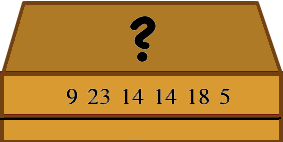
\includegraphics[width=0.25\linewidth]{image1}
			\end{figure}
			Van de vier woorden hieronder kan er slechts \'e\'en het toverwoord zijn. Het welke?
			
			\begin{table}[H]
				\centering
				\begin{tabular}{|c c|}
					\hline
					\textbf{A} & BEDDEN \\ 
					\textbf{B} & SCHORS \\  
					\textbf{C} & APPELS \\ 
					\textbf{D} & TUNNEL \\ 
					\hline
				\end{tabular}
			\end{table}
	\end{minipage} \\ \\
	
\end{document}	